\documentclass[11pt]{article}

%\usepackage[utf8]{inputenc}
\usepackage[a4paper, margin=1in]{geometry}


\usepackage{graphicx}
\usepackage{float}
\usepackage{xcolor}
\usepackage{enumerate}

\usepackage{amsthm}

\usepackage{natbib}

\usepackage{hyperref}
\usepackage{float}

\setlength\parindent{0pt}
\setlength\parskip{5pt}

\usepackage{listings}
\lstset{
basicstyle=\small\ttfamily,
columns=flexible,
breaklines=true,,
stepnumber=1,
}

\definecolor{silver}{gray}{0.9}

\theoremstyle{definition}

\newsavebox\notebox
\newtheorem{mynote}{Note}
\newenvironment{note}%
  {\begin{lrbox}{\notebox}%
   \begin{minipage}{\dimexpr\linewidth-2\fboxsep}
   \begin{mynote}}%
  {\end{mynote}%
   \end{minipage}%
   \end{lrbox}%
   \begin{trivlist}
     \item[]\colorbox{silver}{\usebox\notebox}
   \end{trivlist}}

\newsavebox\examplebox
\newtheorem{myexample}{Example}
\newenvironment{example}%
  {\begin{lrbox}{\examplebox}%
   \begin{minipage}{\dimexpr\linewidth-2\fboxsep}
   \begin{myexample}}%
  {\end{myexample}%
   \end{minipage}%
   \end{lrbox}%
   \begin{trivlist}
     \item[]\colorbox{silver}{\usebox\examplebox}
   \end{trivlist}}


\title{File formats in Mobius}
\author{Magnus Dahler Norling}

\begin{document}

\maketitle

\tableofcontents

\section{Introduction}

This document describes how to use the parameter and input file formats that the Mobius framework has built-in functionality to load or generate.

\section{The standard .dat format}

\subsection{General}
The .dat format is the format that is the easiest to work with when setting up index set structure, parameters and inputs for a new dataset. The .dat files are utf-8 encoded text files. We recommend editing them in a plain text editor like Notepad++.

\begin{note}
Unless you are on Windows, you may have trouble using file paths with special characters like \o, \"{o} etc.
\end{note}

\begin{note}
If you find the rest of this section too technical, just skip to the examples.
\end{note}

\begin{enumerate}[i]
\item You can put a comment in one of these files using the \# symbol. This will treat the rest of the line as a comment that is ignored when parsing the file.
\item Quoted strings are sequences of characters enclosed in a pair of quotation marks " ". These can contain contain utf-8 encoded strings, but not newlines.
\item Outside quoted strings, everything has to be ascii.
\item Except for inside quoted strings and except for newlines after a \#, all consecutive sequences of whitespace (space characters, tabulars, newlines) are treated as one single space.
\item Each .dat file is treated as a series of tokens. A token is a sequence of characters that encode one value or symbol. An overview of the types of tokens are given in Table \ref{tab:tokens}.
\end{enumerate}

\begin{table}[H]
\centering
\label{tab:tokens}
\begin{tabular}{|l|c|}
\hline
{\bf Token type} & {\bf Example} \\
\hline
Colon & {\tt :}  \\
\hline
Open brace & {\tt \{} \\
\hline
Close brace & {\tt \}} \\
\hline
Number & {\tt 8} or {\tt 0.05} or {\tt 1e-9} or {\tt NaN} \\
\hline
Boolean &{\tt  true} or {\tt false} \\
\hline
Date & 1999-05-01 (format YYYY-MM-DD) \\
\hline
Time & 12:31:00 (format hh:mm:ss) \\
\hline
Unquoted string & {\tt index\_sets} \\
\hline
Quoted string & {\tt "Timesteps"} \\
\hline
\end{tabular}
\caption{Types of allowed tokens in the standard format}
\end{table}

A \emph{Datetime} is either a Date alone or a Date followed by a Time.

Both quoted strings and unquoted strings are always case sensitive, so you can for instance not type "landscape units" if you want to talk about the index set "Landscape units".

\subsection{The parameter file}

\begin{example}\label{ex:parameterfile}
A shortened example of a parameter file
\begin{lstlisting}
index_sets :
# You can add in as many landscape units as you like,
# but remember to fill in corresponding parameter values!
"Landscape units" : {"Forest" "Agricultural"}
"Soils" : {"Direct runoff" "Soilwater" "Groundwater"}
"Reaches" : {"Reach 1" {"Reach 2" "Reach 1"}}

parameters :
"Timesteps" :
365

"Start date" :
1999-1-1

"Growing degree threshold" :
1 2.0

"Percolation matrix" :
0.2 0.8 0.0
1.0 0.5 0.5
0.0 0.0 1.0

0.1 0.9 0.0
1.0 0.6 0.4
0.0 0.0 1.0

"Reach has effluent input" :
false true

"%" :
9 81
33.0 67.0
\end{lstlisting}
\end{example}

Every parameter file, like the file in Example \ref{ex:parameterfile}, needs to have two sections (in that order)
\begin{enumerate}[i]
\item {\tt index\_sets :} This section describes the indexes of each index set that is present in the model. Here you can for instance configure the number of landscape units or reaches in your dataset.
\item {\tt parameters :} This section lets you fill in values for individual parameters. If a parameter indexes over one or more index set, you need to provide a number of values corresponding to the number of (tuples of) indexes.
\end{enumerate}

\subsubsection{Index sets}
Which index sets that are present are determined by the model you want to run. Most often you are free to determine which indexes  they have, but sometimes, the indexes of an index set are also specified by the model. For instance, INCA-N requires you to have the indexes \{"Direct runoff" "Soilwater" "Groundwater"\} for soils. In any case, you have to provide a set of indexes for each index set in the parameter file. There are two types of index sets, basic and branched.
\begin{enumerate}[i]
\item Basic index sets are index sets with no additional structure except for the order of the indexes. One example is "Landscape units" in Example \ref{ex:parameterfile}. To provide the indexes of a basic index set, type the quoted name of the index set followed by a colon and a brace-enclosed space-separated (no commas) list of the quoted names of the indexes.
\item In a branched index set, each index can have zero or more branch inputs, where each input is another index. In distributed catchment models this is used to encode a river network of reaches, where each reach can be an input to other reaches. The indexes of a branched index set are provided as a brace-enclosed list of items, where each item is either a quoted name of an index or a brace-enclosed list of quoted names of indexes. If the item is a name appearing alone, it signifies an index that does not have any inputs. If an item is a list, the first string of the list is a new index, and the rest of the strings are names of previously declared indexes that are inputs to this one.
\end{enumerate}

\begin{example}
The river system has reaches "R1", "R2" and "R3", where "R1" is an input to "R2" and "R2" is an input to "R3".
\begin{lstlisting}
"Reaches" : {"R1" {"R2" "R1"} {"R3" "R2"}}
\end{lstlisting} 
\end{example}

\begin{example}
The river system has reaches "R1", "R2" and "R3", where "R1" and "R2" have no inputs of their own, but are both inputs to "R3" (forming a Y-like shape).
\begin{lstlisting}
"Reaches" : {"R1" "R2" {"R3" "R1" "R2"}}
\end{lstlisting} 
\end{example}

\begin{example}
The river system consist of three separate reaches "R1", "R2" and "R3", where none of them are inputs to any others. This could potentially happen if you want to simulate three separate streams at the same time that for instance are inputs to a lake (where the lake itself is not modelled by this framework).
\begin{lstlisting}
"Reaches" : {"R1" "R2" "R3"}
\end{lstlisting} 
\end{example}

\subsubsection{Parameters}

The parameter section consists of a series of quoted names of parameters followed by their values. Any parameter in the model will have one of four types (that are specified by the model). 

\begin{table}[H]
\centering
\label{tab:parametervalues}
\begin{tabular}{|l|c|}
\hline
{\bf Parameter type} & {\bf Example value} \\
\hline
{\bf double} & {\tt 8} or {\tt 0.05} or {\tt 1e-9} or {\tt NaN}  \\
\hline
{\bf uint} & {\tt 10} \\
\hline
{\bf boolean} &{\tt  true} or {\tt false} \\
\hline
{\bf time} & {\tt 1999-1-1} \\
\hline
\end{tabular}
\caption{Parameter value types}
\end{table}

\begin{enumerate}[i]
\item Parameter values of type {\bf double} (double-precision floating point numbers) can written as numbers with or without a decimal separator '.', or in scientific notation. Technically you could also provide a NaN (not-a-number), but that will probably crash the model in most cases.
\item Values of type {\bf uint} (unsigned integers) have to be written as a non-negative number without any commas. These are often used to denote a number of timesteps or days of duration for some process.
\item {\bf Boolean} values are either {\tt true} or {\tt false}. These are typically switches that turn on or off a process.
\item Values of {\bf time} type are provided as a date on the format yyyy-mm-dd.
\end{enumerate}

Every parameter indexes over a list of index sets determined by the model. Note that an index set can appear more than one time in this list. If a parameter indexes over no index sets, it has only one value. If it indexes over one index set it has one value for each index in that index set. If it indexes over more than one index set, it has one value for each element in the cartesian product\footnote{Remember that the Cartesian product of sets $X$ and $Y$ is the set of tuples $(x, y)$, with $x\in X$ and $y\in Y$.} of these index sets, i.e. the number of values is equal to the product of the number of indexes.

In the following examples, the index sets are as in Example \ref{ex:parameterfile}. These examples will also describe the order that the values should appear in.

\begin{example}
The parameter "Timesteps" does not index over any index sets, so it has only one global value.
\begin{lstlisting}
"Timesteps" :
365
\end{lstlisting}
\end{example}

\begin{example}
The parameter "Growing degree threshold" indexes over the index set "Landscape units", which has two indexes "Forest" and "Agricultural". "Growing degree threshold" thus has two values.
\begin{lstlisting}
"Growing degree threshold" :
1 2.0
\end{lstlisting}
Here {\tt 1} is the value for "Forest", while {\tt 2.0} is the value for "Agricultural".
\end{example}

\begin{example}
The parameter "\%" indexes over the index sets "Reaches" and "Landscape units" (the order of these are important), both having two indexes. "\%" thus has 4 values. Which reach you are in is indicated by the row, while which landscape unit is indicated by the column.
\begin{lstlisting}
"%" :
9 81
33.0 67.0
\end{lstlisting}
Here {\tt 9} is the value for \{"Reach 1" "Forest"\} (signifying that the catchment of reach 1 has a 9\% forest cover). Similarly, \{"Reach 1" "Agricultural"\} is 81, \{"Reach 2" "Forest"\} is 33.0 and \{"Reach 2" "Agricultural"\} is 67.0
\end{example}

\begin{example}
The parameter "Percolation matrix" indexes over the index sets "Landscape units", "Soils" and "Soils" (Soils appearing twice). "Landscape units" has 2 indexes, while "Soils" has 3, so "Percolation matrix" has $2*3*3=18$ values.
\begin{lstlisting}
"Percolation matrix" :
0.2 0.8 0.0
1.0 0.5 0.5
0.0 0.0 1.0

0.1 0.9 0.0
1.0 0.6 0.4
0.0 0.0 1.0
\end{lstlisting}
The landscape unit signifies which block matrix you are in (the first block matrix is for "Forest", the second for "Agricultural"). The first soil index is the row, while the second is the column. In this case, the "Percolation matrix" of each landscape unit appears exactly as they are specified in the PERSiST model \cite{futter14}.
\end{example}

The general rule for the order values appear in is that you index over the rightmost index set first, then the next to the left, then the next to the left and so on.

\begin{note}
It is the order that the values appear in that is important. You could remove the newlines between value rows. The newlines are only there for visual clarity for a human editor.
\end{note}

If you provide the name of a parameter, you have to provide all of its values. However, you can omit a parameter from the file entirely. In that case, that parameter will get its model-specified default value.

Usually you will work with parameter files that have been autogenerated by the model. In that case, the files will contain useful comments about which parameters index over which index sets, what are their units and model-recommended min and max values, and often a description of the parameters.

\begin{example}
A shortened example of an autogenerated parameter file
\begin{lstlisting}[mathescape]
# Parameter file generated for PERSiST V1.1 at 2019-02-11 15:30:40

index_sets :
"Landscape units" : {"Forest" "Agricultural"}
"Soils" : {"Direct runoff" "Soilwater" "Groundwater"}
"Reaches" : {"Reach 1" {"Reach 2" "Reach 1"}}

parameters :
###################### (no index sets) ######################
"Timesteps" :     #(days) [0, 18446744073709551615]
365

"Start date" :     # [1000-1-1, 3000-12-31]
1999-1-1

###################### "Landscape units" ######################
"Growing degree threshold" :     #(${^\circ}$C) [-4, 4] The temperature at or above which plant growth and hence evapotranspiration are assumed to occur
1 2

###################### "Landscape units" "Soils" "Soils" ######################
"Percolation matrix" :     #(dimensionless) [0, 1]
0.2 0.8 0.0
1.0 0.5 0.5
0.0 0.0 1.0

0.1 0.9 0.0
1.0 0.6 0.4
0.0 0.0 1.0

###################### "Reaches" ######################
"Reach has effluent input" :
false true

###################### "Reaches" "Landscape units" ######################
"%" :     #(%) [0, 100] The percentage of a subcatchment occupied by a specific land cover type
9 81
33.0 67.0
\end{lstlisting}
\end{example}

\subsection{The input file}\label{sec:datinput}

\begin{example}\label{ex:inputfile}
A shortened example of an input file
\begin{lstlisting}
start_date :
1999-1-1

timesteps :
5

additional_timeseries :
"Discharge"

index_set_dependencies :
"Actual precipitation" : {"Reaches"}
"Discharge" : {"Reaches"}

inputs :

"Air temperature" :
-10.7251
-18.1251
-14.8251
-23.6251
-24.7251

"Actual precipitation" {"Reach 1"} :
2.75
3.3
2.75
15.07
8.03

"Actual precipitation" {"Reach 2"} :
1.54
1.65
0.88
7.15
1.54

"Discharge" {"Reach 1"} :
1999-01-01	0.001982
1999-01-02	0.001982
1999-01-04	0.001428
1999-01-05	0.00404

"Discharge" {"Reach 2"} :
1999-01-01	0.001486
1999-01-03	0.003005
1999-01-05	0.002082

\end{lstlisting}
\end{example}

Input files, like the file in Example \ref{ex:inputfile}, can or must have the following sections
\begin{enumerate}[i]
\item {\tt start\_date :} (optional) The start date of the input data. This can be earlier or equal to the model run start date that is provided by the "Start date" parameter in the parameter file. If this section is not in the input file, the input start date will be assumed to be equal to the model run start date.
\item {\tt timesteps :} or {\tt end\_date} (required) The {\tt timesteps} is the number of values that you wish to allocate for each input series. You have to provide enough timesteps to cover the entire model run, meaning that the input start date plus the input timesteps must be greater than or equal to the model run start date plus the model run timesteps. Alternatively, you can instead provide an {\tt end\_date}. The number of time steps is then computed using the model time step resolution. The end date is inclusive.
\item {\tt additional\_timeseries :} (optional) Here you must declare the name of additional timeseries that you want to put into the dataset, that are not required by the model. This is for instance used to be able to load measured comparison data for viewing together with the model results in MobiView, or for use in calibration routines. The data itself is put in the {\tt inputs} section just like the other time series.
\item {\tt index\_set\_dependencies :} (optional) If one or more of your timeseries varies over some of the model index sets, you have to declare so here. For instance, you can choose whether or not you have an "Air temperature" timeseries that is the same for every subcatchment, or if you have a separate timeseries for each reach. You can add dependencies on multiple index sets at the same time, so "Air temperature" could depend on both "Reaches" and "Landscape units" (not that that is likely), but if you do something too crazy you may break the model. This is because the model may adapt to evaluate equations such as "Precipitation falling as snow" to evaluate for every index you have a precipitation and air temperature timeseries for, and this will propagate to evaluations of other equations that depend on the value of "Precipitation falling as snow". Generally you should be safe if you do something that feels sensible, such as having one timeseries per reach.
\item {\tt inputs :} (required) The actual input data. If you did not declare any index set dependencies for an input, you only provide one timeseries. Otherwise you provide one for each (combination of) index(es) in the index set(s) it depends on.
\end{enumerate}

You can completely omit providing data for a timeseries (i.e. don't type its name or any values for it). In that case it will be asumed to be equal to 0 for every timestep. There are two formats you can choose.
\begin{enumerate}[i]
\item If you use the dense format, just list all the values after one another. If you use this format you have to provide exactly as many values as the number of timesteps you declared for the input data.
\item If you use the sparse format, list pairs of dates (format yyyy-m-d) and values. The dates do not have to be provided in order.
\end{enumerate}
Input values can be provided in the same format as parameters of type double in the parameter file. I.e. they can be numbers with or without decimal separator or in scientific notation.

\begin{note}
If you have a timeseries of that you want to use as a model input timeseries (as opposed to an additional observation timeseries) and it has missing values, you have to do preprocessing on it yourself to interpolate the missing values before you put it in the input file. Alternatively, you can use the in-built linear interpolation as specified below.
\end{note}

\begin{note}
Additional timeseries (ones not specified by the model) are by default cleared to NaN instead of to 0. This is for instance useful when using this feature to load in observation series, because it means that dates you don't provide values for will be properly treated as missing values.
\end{note}

There are a few more advanced options you can use when providing inputs.

\begin{example}\label{ex:declarewithunit}
Declaring a unit for an additonal timeseries.
\begin{lstlisting}
additional_timeseries :
"Discharge" unit "m3/s"
"Nitrate concentration"      #NOTE: you can freely declare units for some timeseries while omitting them for others
\end{lstlisting}
\end{example}

\begin{example}\label{ex:multiseries}
Providing the same timeseries for multiple (combinations of) indexes at the same time
\begin{lstlisting}
"Actual precipitation" {"Reach 1"} {"Reach 2"} :
1.54
1.65
0.88
7.15
1.54

"Actual precipitation" {"Reach 3"} {"Reach 4"} :
2.75
3.3
2.75
15.07
8.03

"Fertilizer nitrate" {"Reach 1" "Agricultural"} {"Reach 2" "Agricultural"} {"Reach 3" "Agricultural"} :
0.4
0.4
0.5
0.5
0.6
\end{lstlisting}
\end{example}

As in Example \ref{ex:multiseries} you can make sure the same timeseries is used in more than one, but typically not all, instances (if you wanted one series to be used in all instances, you would just not give it an index set dependency).

\begin{example}\label{ex:constantperiods}
Declaring constant periods of values
\begin{lstlisting}
"Nitrate dry deposition" :
1999-01-01 to 1999-05-31 0.01
1999-06-01 to 1999-12-31 0.02
\end{lstlisting}
\end{example}

As in Example \ref{ex:constantperiods} you can declare that the timeseries should have a given constant value between two dates. Both the start date and end date is inclusive. Note that this otherwise counts as using the sparse format. Moreover, the periods do not have to be declared in order. You can also combine these advanced features freely as seen below.

\begin{example}
Combining various advanced formats.
\begin{lstlisting}
"Nitrate dry deposition" {"Reach1"} {"Reach2"}:
1999-01-01 to 1999-05-31 0.01
1999-06-01 to 1999-12-31 0.02
2000-01-01 0.01    #NOTE: you can provide values for single days in-between periods
2000-01-02 0.015
1999-01-03 to 1999-05-31 0.01
\end{lstlisting}
\end{example}

\subsubsection{Interpolation}\label{sec:dat-interpolate}

If you have a time series with missing values and you want the model to fill them with interpolated values, you can specify that in the input file.

\begin{example}
Linear interpolation of time series.
\begin{lstlisting}
"Nitrate dry deposition" {"Reach1"} {"Reach2"} linear_interpolate:
1999-01-01 0.01
1999-06-01 0.02
2000-01-01 0.01   
2000-07-02 0.015
\end{lstlisting}
\end{example}

When you use interpolation, you can not use the {\tt to} directive to specify a constant interval, but you can instead do it by having two subsequent dates with the same value. Moreover, all dates in the list have to be sequentially increasing. Any dates before the first date in the provided list or after the last date will be given the constant value of the first date or the last date respectively unless the {\tt inside} flag is set.

The following flags are supported
\begin{enumerate}
\item {\tt step\_interpolate}. Fill each given value (as a constant) for all dates until the next date where a value is specified.
\item {\tt linear\_interpolate}. Fill a linear interpolation of values between dates where values are specified.
\item {\tt inside}. Only interpolate between given values. If this is flag is  {\bf not} specified, the dates up to the first given value are filled with the first given value, and the dates after the last given value are filled with the last given value. Can be combined with any of the interpolation types.
\end{enumerate}
If you want to set multiple flags, just put them after one another with a space in between.

\subsubsection{Yearly repetition}\label{sec:dat-yearly-repeat}

You can make an input time series repeat the same pattern each year. The data provided for the first year of the input data interval is repeated for all of the other years.

\begin{example}
Yearly repetition.
\begin{lstlisting}
"Fertilizer nitrate" {"Agricultural"} repeat_yearly :
1990-04-25 to 1990-05-04	6
1990-06-10 to 1990-06-19	0.75
1990-09-01 to 1990-09-10	0.75
\end{lstlisting}
\end{example}

The {\tt repeat\_yearly} flag can be combined with interpolation. In that case, the interpolation is applied first, then the resulting first year is repeated across the series.

\subsubsection{Including multiple input files}

If you have a lot of input data, it can be useful to organize it in many separate files. You need to have one master file that has all the "organisational" data. Then below the {\tt inputs} section in the master file, you can use an {\tt include\_file} directive to read timeseries from another file. The other file has to contain one or more entire timeseries (including the heading name and optional indexes). The path of the file you include should be relative to the location of the master file.

\begin{example}
Including other files. The master file:
\begin{lstlisting}
start_date : 2004-01-01
timesteps  : 5

inputs:

include_file "depositions.dat"

"Air temperature":
-10.7251
-18.1251
-14.8251
-23.6251
-24.7251
\end{lstlisting}
The entire contents of depositions.dat:
\begin{lstlisting}
"Nitrate dry deposition" :
2004-01-01 to 2005-01-01 0.01
2005-01-02 to 2008-01-01 0.02

"Nitrate wet deposition" :
2004-01-01 to 2005-01-01 0.03
2005-01-02 to 2008-01-01 0.04
\end{lstlisting}
\end{example}

\begin{note}
All organisational data like additional timeseries or index set dependencies have to be declared in the master file even though the information may be about timeseries that are included from separate files.
\end{note}

\subsubsection{Models with non-daily timesteps}

Mobius now supports models that have step sizes that are measured in seconds, minutes, hours, days, months or years. If a model has a timestep that is less than a day, one can use the full Datetime format to give a time value. Note that a given compiled model is always just using one timestep size, so you should find out what that is before making parameter and input files for it (most example models for Mobius still use a daily step size). We still use the term "start date" instead of "start time" for legacy reasons.

\begin{example}
Usages of the datetime format
\begin{lstlisting}

start_date : 1990-01-15 12:00:00

"Air temperature" :
1990-01-15 12:00:00  5.1
1990-01-15 13:00:00 to 1990-01-15 16:00:00 7.8
\end{lstlisting}
\end{example}

A Datetime can similarly be used for the model "Start date" parameter in the parameter file. There are some important rules to consider:
\begin{enumerate}[i]
\item "1990-04-03" is equivalent to "1990-04-03 00:00:00".
\item A start date refers to the beginning of the first timestep. The timestep itself is an interval starting at some timestamp and spanning one step size.
\item The input start date and the model run start date have to be aligned so that the the model run start date is either zero or a full number of timesteps after the input start date.
\item If a value in an input series is given a timestamp that is not perfectly aligned with the beginning of a timestep, it will be considered to belong to the timestep whose interval the timestamp is in. For instance, in a model with an hourly timestep, a value given a timestamp of 12:53:14 will be considered to belong to a timestep starting at 12:00:00 (given that the start date was at a whole hour).
\item If more than one value is given for the same timestep, only the last one is used. This means that if you feed hourly data to a daily-timestep model, only the last value of each day is used.
\item No processing, aggregation or interpolation is done to the data by Mobius by default (unless if you specify interpolation). This is because this is something that should be done with care by the researcher and often has to be done differently for different types of data. There is no one-size-fits-all way to automate it without potentially causing mistakes or confusion.
\item Timeseries given in the dense format are always considered to be aligned with the timesteps of the model.
\end{enumerate}

In models that have their timestep measured in months or years, the timestep will always be full calendar months or calendar years. Note that this means that the length of each timestep (if measured in e.g. days) changes with the step since months and years are not of equal length. Models such as these have to have start dates (both in the parameter and input file) set at the first day of some month. For instance 1990-05-01 is a valid start date for such a model, but 1990-05-05 is not.


\subsubsection{Converting from .csv or .xlsx}
In many cases, your input data will a priori exist in a .csv format or an .xlsx format. Since there are very many ways your data could be formatted it would be difficult for us to make a converter that can handle every possibility. If you don't know any python or other scripting languages you could use to convert them, you may have to learn some tricks. We will just give some quick tips here. A more complete tutorial may be for the future.

\begin{enumerate}[i]
\item If your data are opened in Excel (or Open Office Calc) your can click the letter of a column in the top bar to select the entire column, then ctrl-c to copy it. You can now paste it in a text editor.
\item You need all values to have a '.' decimal separator rather than a ','. You can either do a search-replace in a text editor after copying the values, or in excel go to File$\rightarrow$Options, On the Advanced tab, under Editing options, uncheck the Use system separators box, then type in the right Decimal separator in its box.
\item To format a column of dates to the yyyy-m-d format, select the colum, then right click it and select Format Cells. Under Date select the right format.
\item If you have one date column and many data columns and you want to copy just the date column together with one data column, you can temporarily copy the data column next to the date column and ctrl-select and copy the two together.
\end{enumerate}

\subsection{Error messages}

Most often if you get an error during the parsing of a parameter or input file, it will tell you at which line and column in the file that the error happened. Here is a non-exhaustive list of error messages you could encounter.

\begin{example}
The message:
\begin{lstlisting}
ERROR: In file langtjernparameters.dat line 4 column 1: The index set "landscape units" was not registered with the model.
\end{lstlisting}
The culprit line:
\begin{lstlisting}
"landscape units" : {"Forest" "Wetland"}
\end{lstlisting}
Explanation: The model only recognizes "Landscape units" as the name of one of its index sets. This is case sensitive.
\end{example}

\begin{example}
The message:
\begin{lstlisting}
ERROR: In file langtjernparameters.dat line 5 column 75: Found a token of unknown type.
\end{lstlisting}
The culprit line:
\begin{lstlisting}[mathescape]
"Soils" : {"Direct runoff" "Organic layer" "Mineral layer" "Groundwater"} $\ae$
\end{lstlisting}
Explanation: '\ae' is not a valid token (though you can still use that character inside quoted strings if you want to).
\end{example}

\begin{example}
The message:
\begin{lstlisting}
ERROR: In file langtjerninputs.dat line 12 column 27: Did not get the right amount of indexes for input Air temperature. Expected 2, got 1.
\end{lstlisting}
The culprit line:
\begin{lstlisting}[mathescape]
"Air temperature" {"Bork"}:
\end{lstlisting}
In this case you have declared "Air temperature" to depend on either 2 index sets.
\end{example}

\begin{example}
The message:
\begin{lstlisting}
ERROR: In file langtjerninputs.dat line 12 column 27: The index "Bork" was not registered with the index set "Reaches".
\end{lstlisting}
The culprit line:
\begin{lstlisting}[mathescape]
"Air temperature" {"Bork"}:
\end{lstlisting}
In this case you have declared "Air temperature" to depend on the index set "Reaches", but "Bork" is not one of the indexes you provided for that index set in the parameter file.
\end{example}

\section{The spreadsheet format}

\subsection{General}

The spreadsheet format is very convenient to edit by hand, but is only available to users on a Windows machine who have Excel installed. This format only exists for input data, not for parameter data.

\subsection{The input file}

The input file has to be a single Excel .xlsx file. You can have as many tabs (sheets) as you want in the file, and all of them will be read in by default. If you want to make Mobius ignore a tab (useful if you want to keep a tab for documentation or as a scratchpad), put {\tt NOREAD} in cell A1 of that tab (apart from that it doesn't matter what you put in A1).

\begin{note}
The names of the tabs are ignored. Any color coding or borders are also ignored, so you can use these to enhance human readability if you want to.
\end{note}

Each sheet consists of a header and a data block. The header contains information about what time series the sheet contains (and any additional info about them), while the data block contains the actual values of the series.

In the easiest example, the header is just the first row and contains the names of some input series. The names have to start in cell B1 and continue along row 1 with one column per name. All names should be formatted as text (this is usually automatic).

In the data block, column A has to be filled with dates, and can not have any empty cells between dates.

\begin{figure}[h]
\centering
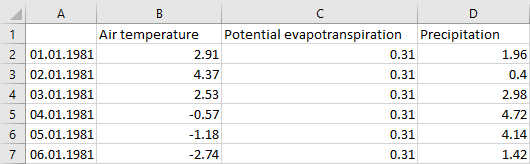
\includegraphics[width=0.7\linewidth]{img/excel_simple}
\caption{A simple spreadsheet example.}
\end{figure}

The dates have to be formatted as \emph{Date} or \emph{Text} (this is usually automatic, but if not you can select the column, right click, and choose "format cells"). If they are formatted as text, they have to be on the form {\tt YYYY-MM-DD} explained in the {\tt .dat} format. If they are formatted as dates, the format displayed in the Excel sheet can be whatever you want.

\begin{note}
Note that Exel does not support date formatting for dates earlier than 1900-1-1, so they have to be put as text. Moreover dates in the year 1900 can have a buggy internal format when formatted as a date, so it is safer to format them as text.
\end{note}

The range of input data that is allocated for the dataset will be the range of all dates given across all the tabs. This means that you can e.g. have a tab with observed data that has a shorter date range than the tab with the model inputs. Mobius will figure out how much space it needs to allocate for them. Date ranges can also have missing dates (but not empty cells).

In the values block you can have empty cells, but this is (unless the model handles this specifically) only recommended for observed series, not for series required by the model. Missing values or entire missing time series are treated the same way as in the {\tt .dat} format (see Section \ref{sec:datinput}). Values should be formatted as \emph{Number} or \emph{Text}.

Any input name that is not recognized as a model input by the model will be treated as an \emph{additional time series}, and will be loaded in so that you can e.g. use it as a comparison calibration series in MobiView.

\begin{note}
Cell values can be results of Excel formulas. Mobius will read the value resulting from the formula, not the literal formula.
\end{note}

\subsubsection{Indexing}

If you want to index a time series over multiple indexes (for instance to provide a separate series per "Reach" or "Landscape unit"), must put one row below row 1 per index set you want to use . These rows have to have the name of the index set in cell A.

\begin{figure}[h]\label{fig:excel-indexed}
\centering
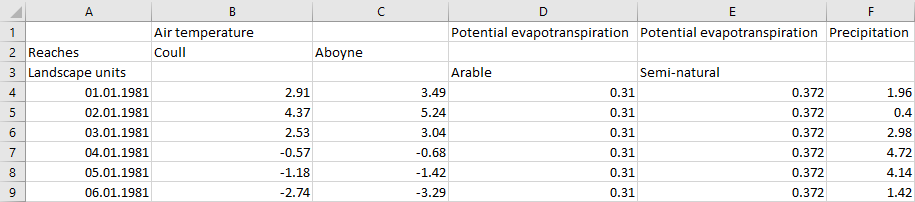
\includegraphics[width=0.95\linewidth]{img/excel_indexes}
\caption{A spreadsheet example with indexed inputs.}
\end{figure}

If you put an empty cell in the input name row, that column will be treated as belonging to the same input name as the last given input name before it on the row. For instance in Figure \ref{fig:excel-indexed}, both column B and C are "Air temperature" columns.

If you put an index name in the header in the row belonging to an index set and a column belonging to an input name, that input is treated as indexing over that index set, and this particular column is assigned to that index. For instance in Figure \ref{fig:excel-indexed}, "Air temperature" is indexed over "Reaches", "Potential evapotranspiration" is indexed over "Landscape units", and "Precipitation" is not indexed over anything (just having one "global" series). You can also make a series index over multiple index sets by putting one index per set. Note that all instances of the same input name have to index over the same index sets.

\subsubsection{Interpolation and other modifiers}

In the header you can optionally put a {\emph flags} row below all the other header rows, right above the data block. The A cell of this row has to be empty (and has to be the only empty cell in column A except for potentially A1 and cells at the bottom of the document). In the flags row you can put modifier flags in the columns of the input series (you can have separate flags per series)

The flags {\tt step\_interpolate}, {\tt linear\_interpolate}, {\tt inside} and {\tt repeat\_yearly} work exactly as in the {\tt .dat} format (Sections \ref{sec:dat-interpolate} and \ref{sec:dat-yearly-repeat}).

If you want to combine multiple flags for the same series you provided them with spaces between them inside the same cell.

For \emph{additional time series} you can also provide a unit in the flag cell by writing it as {\tt [unitname]} (the {\tt unitname} can not have spaces in it). (For model input series units are ignored since the model usually specifies the units of its input series, but you could put units there as documentation).

\begin{figure}[h]\label{fig:excel-flags}
\centering
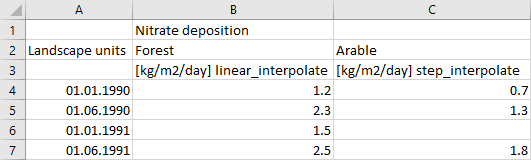
\includegraphics[width=0.6\linewidth]{img/excel_flags}
\caption{A spreadsheet example with flags.}
\end{figure}

You can use flags also if you don't need indexing, in that case the flags row is the row right below the input name row (the flags row in this case is row 2).

\section{The Json format}

\subsection{General}

Json (Javascript object notation)  is another text format that follows a standard that is recognized by many programming language libraries and applications. This format is typically used to serialize the dataset, for instance in order to easily read it from other programs or send it over the web. The reason this is not used as the standard format is that it is less convenient for manual editing and does not support having comments. It is also much slower to load than the other formats, and does not support features like interpolation. Moreover, this is not included by default in builds of Mobius, and can only be used if you compile the models yourself.

\subsection{The parameter file}
The format of the parameter file is similar to the dat format. Apart from having to obey the json standard, the file has to obey a structure similar to that given in Example \ref{ex:jsonpar}

\begin{example}\label{ex:jsonpar}
The structure of the parameter file in json
\begin{lstlisting}
{
	"index_sets" : {
		"Name of regular index set" : ["index 1", "index 2", "index 3"],
		"Name of branched index set" : [
			["index", "branch input 1", branch input 2"],
			<...etc...>
		]
	},
	"parameters" : {
		"Parameter 1" : [1, 2, 3],
		"Parameter 2" : [true, false],
		<...etc...>
	}
}
\end{lstlisting}
\end{example}

\begin{enumerate}[i]
\item The file is a dictionary containing two keys, {\tt "index\_sets"} and {\tt "parameters"}.
\item The value of {\tt "index\_sets"} is a dictionary where every key is the name of an index set.
\item The value of a basic index set is a list of the names of its indexes.
\item The value of a branched index set is a list of lists, where every sub-list is first the name of an index and then all the branch inputs to that index.
\item The value of {\tt parameters"} is a dictionary where every key is the name of a parameter.
\item The value of every parameter is a list of values. These values are given in the same order as in the .dat format (but have to be comma separated as per the json standard).
\end{enumerate}

\subsection{The input file}
The format of the input file is similar to the dat format. Apart from having to obey the json standard, the file has to obey a structure similar to that given in Example \ref{ex:jsonin}

\begin{example}\label{ex:jsonin}
The structure of the input file in json
\begin{lstlisting}
{
	"creation_date": "2019-03-07 12:36:29",
	"additional_timeseries": [
		"Observed discharge"
	],
	"index_set_dependencies" : {
		"Air temperature" : ["Reaches"]
	},
	"start_date": "1981-01-01",
	"timesteps": 10
	"data": {
		"Air temperature": [
			{
				"indexes": ["Reach 1"],
				"values": [1, 2, 3, 4, 5, 6, 7, 8, 9, 0]
			},
			{
				"indexes": ["Reach 2"],
				"values":  [1, 2, 3, 4, 5, 6, 7, 8, 9, 0]
			},
		],
		<...etc...>
	}
}
\end{lstlisting}
\end{example}

\begin{enumerate}[i]
\item The file is a dictionary containing 6 keys, {\tt creation\_date}, {\tt additional\_timeseries}, \\{\tt index\_set\_dependencies}, {\tt start\_date}, {\tt timesteps} and {\tt data}.
\item {\tt creation\_date} is optional and its value is a string containing the time the file was created (if it was autogenerated).
\item The value of {\tt additional\_timeseries} is a list of names of additional input timeseries.
\item The value of {\tt index\_set\_dependencies} is a dictionary where every key is the name of an input. The value associated to every key is a list of names of index sets.
\item The value of {\tt start\_date} is a string with a date on the format "y-m-d".
\item The value of {\tt timesteps} is a number.
\item The value of {\tt inputs} is a dictionary where every key is the name of an input.
\item The value of every input in {\tt data} is a list of dictionaries. Each of these dictionaries has the two keys {\tt indexes} and {\tt values}. The value of {\tt indexes} is a list of names of indexes for this timeseries. The value of {\tt values} is a list of numeric values. Unlike in the dat format, {\tt NaN} is not a valid json identifier, so {\tt null} is used to signify a missing value instead.
\end{enumerate}

\bibliographystyle{plain}
\bibliography{citations}

\end{document}


